\chapter{Discussion}

\subsection{Integrated Statistical Uncertainty on Fragmentation Function Ratio}
For the purpose of giving a single number to quantify how similar pp and \pPb~ fragmentation functions are, an integrated statistical uncertainty on the ratio of the two was calculated (note: the p-value calculated from the two distributions only indicates that the null hypothesis, pp and \pPb~ are the same, cannot be rejected). First, the fragmentation function in pp was integrated, and the statistical errors were added in quadrature. The summed statistical uncertainty was then divided by this integral to obtain the relative uncertainty. The same was done for the \pPb~ fragmentation function. Then, the two relative uncertainties were added in quadrature and the ratio of the integrals was taken. This is shown in equation~\ref{eq:fragErrorRatio} below,

\begin{equation}\label{eq:fragErrorRatio}
\begin{split}
    I &= \sum_i y_i\cdot z_i \\
    \delta_\mathrm{abs.} &= \delta_0 \oplus \delta_1 \oplus ...\delta_n\\
    \delta_\mathrm{rel} &= \frac{\delta_\mathrm{abs.}}{I},\\
\end{split}
\end{equation}{}

where $I$ is the integral of the fragmentation function, $y_i$ is the conditional yield of associated hadrons in \zt~ bin i, and $z_i$ is the width of \zt~ bin i. Additionally, $n$ is the number of \zt~ bins, and $\delta_i$ is the statistical uncertainty of the ith \zt~ bin. $\delta_\mathrm{rel}$ is the relative statistical error on the fragmentation function. Taking the ratio of the integrals and summing the uncertainties from pp and \pPb~ in quadrature:

\begin{equation}
    \delta_\mathrm{ratio} = \frac{I_\mathrm{p-Pb}}{I_\mathrm{pp}}\cdot (\delta_\mathrm{rel,pp} \oplus \delta_\mathrm{rel,p-Pb}),
\end{equation}

yields a total integrated statistical uncertainty on the ratio, $\delta_\mathrm{ratio}$ of 13\%. Thus, modifications to the fragmentation function in \pPb are constrained to be less than 13\%.


\section{Kinematic Range Probed}

In this work, azimuthal correlations of charged hadrons with isolated photons, $\gammaiso$, are presented in \pPb~and pp collisions with a center-of-mass energy of \sqrtsNN~ = 5.02 TeV. Isolated photons are measured at midrapidity, {$|\eta|<0.67$}, and with transverse momenta in the range $12 <\pt<40$ \GeVc, which yields the scaling variable {$x_{\mathrm{T}} = 2\pt/\sqrt{s_{\mathrm{NN}}}\ = $ 0.005--0.016}. This $x_{\mathrm{T}}$ range is similar to RHIC measurements at forward rapidity~\cite{Adare:2011sc}.

This study marks the first study of photon-tagged fragmentation in \pPb collisions at the LHC. A precise measurement of $Q^2$ in heavy ion collisions is not possible without reconstructing all particles in the event. Nonetheless, among the LHC experiments, ALICE is uniquely configured to measure low-\pt charged particles. In the context of jet constituents and total jet \pt, ALICE is capable of measuring hard scatterings with a lower $Q^{2}$ than other LHC experiments. This is of particular interest for studying cold nuclear matter effects, as they are expected to be largest at lower $Q^{2}$. 

The agreement between pp and \pPb in this kinematic range constrains modifications to the parton fragmentation function to be less than the integrated uncertainty of 13\% on the \pPb/pp ratio for $ 0.005 x_{\mathrm{T}} < 0.016$, and partons with \pt that roughly corresponds to the photon \pt measured in this analysis.

\subsection{Insensitivity to Parton Distribution Function}
\ref{sec:pdf_insensitivity} detailed the factorization of the hadronic cross section into the product of the parton distribution function (PDF) and the fragmentation function (FF). A very important question to answer for the study modifications to the fragmentation function in pPb collisions compared to pp collisions is: How do we know if the modifications to the observed $\gamma$-tagged associated yields are due to the PDF, and not in fact modifications to the fragmentation function?

To answer this question, the prompt photon and hadronic cross sections need to be understood, and the importance of measuring  \textit{per-trigger} yields. Because the main observable is the conditional yield of hadrons per photon, modifications to the cross production cross sections cancel. Coupled with the fact the photons should not otherwise be effected by nuclear effects, this measurement is most relevant towards constraining the impact of cold nuclear modification on the parton fragmentation function. Eqn.~\ref{eq:cross_sections} shows the factorized cross sections of photons and hadrons in nuclear collisions:

[prompt photon cross section]

[hadronic cross section in PbPb] (reference the FF section in the introduction \ref{sec:FF}).

With XXX being the nPDF. Because this term is shared between the two cross sections, it's contribution is cancelled when this ratio is taken. As the conditional yield observable is directly proportional to the ratio of these two cross sections, the nPDF are not expected to contribute to the final measurement.

Thus, the answer to the question is: The observable per-trigger hadrons yields is by construction insensitive to the differences between the PDF and nPDF.

\section{Comparison to Theory}
The agreement of the ratio with unity constrains the modification of the fragmentation function to be within the reported error bars. However, careful comparison to relevant theory calculations can yield valuable insight. A theory calculation on $\gamma$-hadron spectra in p+Pb for the same kinematic range as this study was performed in \cite{PhysRevC.103.034911}. The paper includes two models, one based on the modified nuclear PDFs, and another that simulates the formation of a small droplet of QGP in \pPB collisions, the experimental signature of which is described in Sec.~\ref{sec:flow}. The comparison between these calculations and this measurement are shown in Fig.~\ref{fig:FF_model}.
\begin{figure}[htpb]
  \centering
  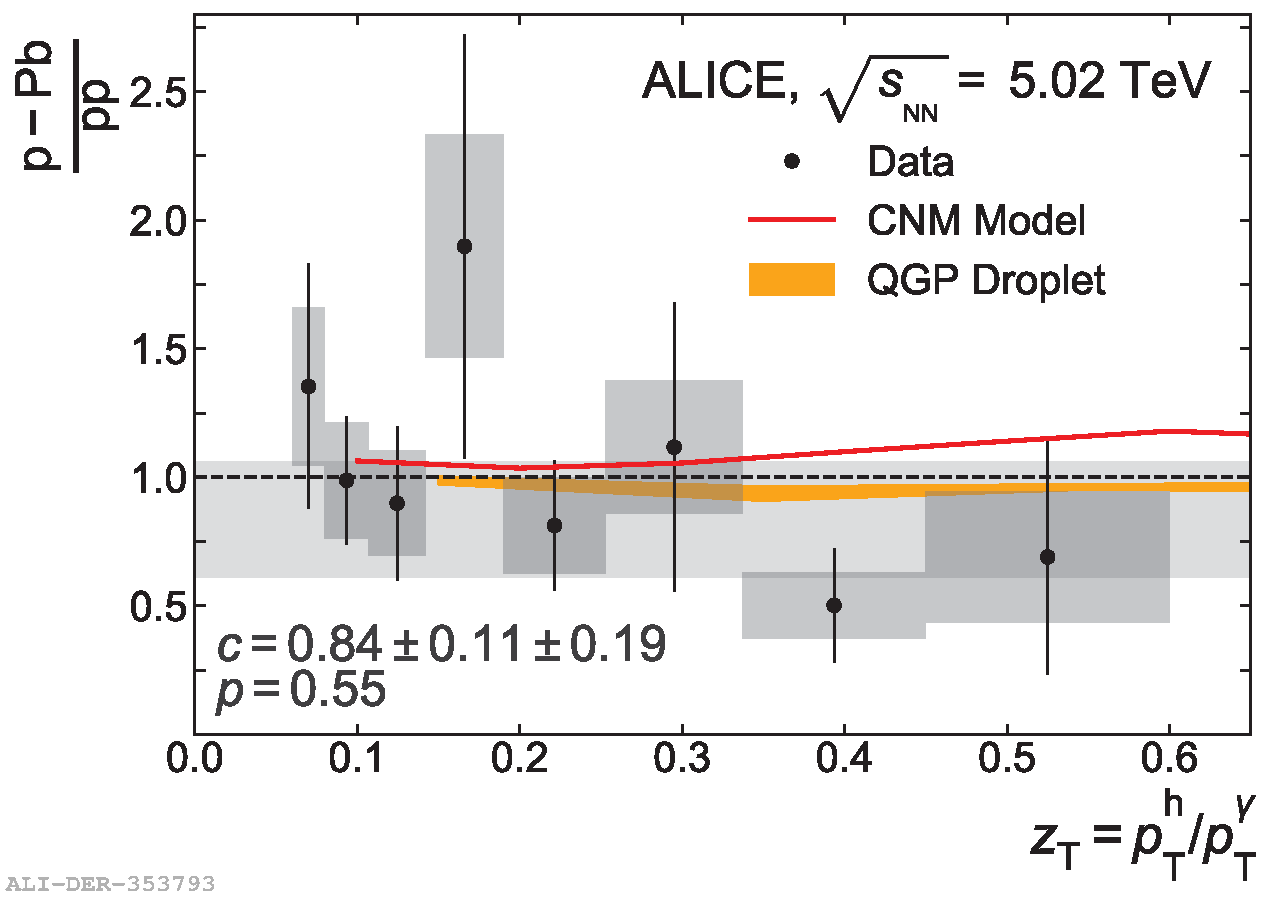
\includegraphics[width=0.8\textwidth]{FF_Model_Comparisons_Ratio.pdf}
  \caption{The ratio of isolated-tagged fragmentation functions for pp and p–Pb data at sqrt(s) = 5.02 TeV as measured by the ALICE detector.  The ratio is compared to two models from \cite{bww{PhysRevC.103.034911}. The cold nuclear matter (CNM) model evolves the partons without parton energy loss, while the quark gluon pasma (QGP) model assumes that a small droplet of QGP is created in p–Pb collisions and applies an energy loss to the partons.}
  \label{fig:FF_model}
\end{figure}

Interestingly, the model predicts that even if a small droplet of QGP were to form, it's effects would be extremely small: it is closer to 1.0 in the ratio than the data, though well within the statistical or systematic uncertainties. Qualitatively, however, the calculation being below unity is inline with qualitative expectations of energy loss in a QGP. While the formation of the QGP is currently a topic of intense debate in the field, this model indicates that the modification of the parton fragmentation function in \pPb~is very unlikely to unambiguously reveal it's existence. The prediction based on nuclear PDFs tells a very different story. It indicates that if a modification to the parton distribution function were to be observed, it should result in an enhancement at higher \zt. 

The data, however is consistent with both models. This is not unsurprising, however, despite the very different underlying physics that make up the models. This observable is designed in its inception to be insensitive to nPDFs, so any model including these effects is expected to be close to unity. As for the QGP droplet, while flow has been observed in small systems, energy loss or jet suppression has not been observed. A common explanation for the observation of flow but not energy loss is that the droplet is too small to significantly modify a parton traversing the tiny droplet. While this remains to be verified, it at least indicates that hot nuclear matter, if present at all, is expected to have a tiny effect on the fragmentation function. This also indicates that if a large modification were to observed in \pPb it is unlikely to be the result of a QGP droplet.

\section{Conclusion}
This analysis marks the first \gammaiso-tagged fragmentation function measurement in \pPb. Furthermore, the relatively lower $Q^2$ probed should include partons that are expected to more sensitive to modification. Nonetheless, no modification is observed when comparing the fragmentation function in \pPb and pp. This means that any modification observed in Pb--Pb that is larger than the integrated uncertainty of 13\% cannot be attributed to cold nuclear matter effects, and must be the modification of the Quark Gluon Plasma on the scattered parton.

An analysis of isolated photon-hadron correlations in Pb--Pb using the same techniques described in this work is a nature next step, one that would focus on hot nuclear matter effects. 

However, for additional insights into cold nuclear matter effects, and their modification to scattered partons, a very different direction is needed. The Electron Ion collider represents this direction, and it will be instrumental in our understanding of the behaviour of QCD in nuclei, as well as in answering fundamental questions of nuclear physics relating to the origin of mass and spin inside the nuclei of hadronic matter that makes up our universe.



